% !TeX root = ../thesis_main.tex

\section{Background Information}\label{sec::backgrund}
The following section provides some basic definitions and principles necessary for the further understanding of this paper and ensures a common level of knowledge of these topics. A formal definition of Agile and DevOps is given, followed by a brief description of the emergence and its current adoption. Next, the basics of virtualization and its usage in a microservice architecture are explained, before the clarification of the connection between microservices, DevOps and familiar tools in a DevOps environment are then pointed out, which forms the end of the chapter.

    \subsection{Modern Software Methodologies}\label{ssec::devops}
    This Section contains a formal definition of agile software development paradigms and the DevOps methodology, explains their connection and points out the fundamental principles of a DevOps enabled culture. These principles and their workflows will be revisited in Section~\ref{sec::solution_concept} as part of the proposed solution concept.
    % \comment{This may be too much and maybe not all of it is needed for the work. Make more compact or remove some of it.}

        \subsubsection{Agile Development}
        \wordhighlight{Agile}, such as the \wordhighlight{V-Model}, \wordhighlight{Waterfall} and \wordhighlight{Prototyping} model, is a software development paradigm. It was proposed and popularized by the \wordhighlight{"Manifesto for Agile Software Development"}, written and published in 2001 by various authors~\cite{manifesto}. Rapid adoption to changes, continuous evolution of software and customer communication are the fundamentals of agile software development.\newline
        The four core principles are:

        \begin{itemize}[label=\(\star\)]
            \setlength\itemsep{0em}
            \item \textbf{Individuals and interactions} over processes and tools
            \item \textbf{Working software} over comprehensive documentation
            \item \textbf{Customer collaboration} over contract negotiation
            \item \textbf{Responding to change} over following a plan
        \end{itemize}

        % Requirements mit s nach dem s
        \noindent Paradigms like Waterfall describe a comprehensive model with an in-depth analysis of requirements and detailed architecture design phase. This results in a fixed and exact sequential schedule for the implementation and testing phase as well as the phase in which the requirements fulfilment is verified. Errors in the requirements analysis or changes in the requirements can cause difficulties in later phases of the project. Agile on the other hand only provides guidelines instead of a complete model. Changes are expected and the project realization is designed to be adaptable. Project phases such as implementation and testing run simultaneously and the entire \ac{SDLC} is shorter and more adaptable \cite{agile_practice}.\newline
        Agile provides a mindset for projects with uncertain or continuously changing requirements. With the increase of software solutions in rapidly changing markets, software requirements also became more uncertain. Accordingly, the agile manifesto became the foundation of several other software development methodologies and frameworks that extend these fundamental guidelines and provide workflows and tooling for the software creation process. Well known exemplary methodologies are \wordhighlight{SCRUM}, \wordhighlight{\ac*{XP}} and \wordhighlight{DevOps}.

        \subsubsection{Definition of DevOps}
        \wordhighlight{DevOps} is a set of practices in software development that aims to increase customer value and software quality by shortening the development life cycle through active collaboration and continuous delivery of improvements \cite{base_devops}, \cite{effective_devops}. The term DevOps is a neologism of development (Dev) and operation (Ops). The combination of these terms is symbolic for the tighter collaboration between the development and operations team, which were strictly separated beforehand. Therefore, DevOps is considered more than just software development principles, it is considered a mindset and company culture. Shorter development times and closer collaboration are the goals of the agile software development paradigm. DevOps builds upon the guidelines and goals of Agile and offers workflows and tools for the software development process for the purpose of an increased user experience value \cite{azuredevops}, \cite{effective_devops}.

        \subsubsection{Principles of DevOps}\label{ssec::devops_princibles}
        In addition to Agile principles, DevOps also extends the \wordhighlight{\acl{XP}} approach by applying its principles to the operations and infrastructure aspects of the application \cite{effective_devops}. The goal is to provide a structured and comprehensive process from coding through testing, packaging and deployment, to operation and monitoring. This process is referred to as a workflow which is made up of several steps. Table \ref{tab::devops_steps} shows an exemplary workflow with a minimum number of steps~\cite{base_devops}.

        \begin{table}[]
            \centering
            \begin{tabularx}{0.85\textwidth}{llX}
                \multicolumn{2}{l}{Step} & Description \\ \midrule\midrule
                1 & \textbf{Coding}& Code development \& review and source control.  \\
                2 & \textbf{Building}& \acs{CI} build and build status.  \\
                3 & \textbf{Testing}& \acs{CI} testing and testing feedback.  \\
                4 & \textbf{Packaging}& Bundle and package to a central registry.  \\
                5 & \textbf{Releasing}& Release management, approvals and automation.  \\
                6 & \textbf{Configuring}& Infrastructure configuration and management.  \\
                7 & \textbf{Monitoring}& Applications performance monitoring.  \\
            \end{tabularx}
            \caption{Common DevOps Workflow Steps. \\\textit{Source:~\cite{base_devops}}}
            \label{tab::devops_steps}
        \end{table}

        \noindent Tasks and activities representing the core process of a DevOps operation emerge with such a workflow. These tasks include configuration management, release management, \ac{CI}, \ac{CD}, infrastructure provisioning, test automation and application performance monitoring~\cite{azuredevops}.
        Generally, it is the overall aim to conduct structuring and optimizing processes on the entire path of the \ac{SDLC}, while also providing the team with appropriate tooling. Even the infrastructure provisioning is structured and automated as its specifications are stored as code, just like application configurations. This approach is referred to as \wordhighlight{\ac{IaC}} \cite{base_devops}. This work will focus on applying this structuring of workflows to the development environments in order to enable homogeneous environments and an efficient development process. For this purpose, tools from the \ac{CI} and \ac{IaC} concepts will be used. \newline
        A DevOps-principled architecture has multiple deployment stages. A staging and live environment is considered the minimal foundation of any such project \cite{azuredevops}. In order to test and operate this deployment stages software teams need to have a reliable and efficient way to manage their infrastructure state and configuration. This is closely related to the \ac{IaC} principle, which describes the provisioning and maintenance process of computing resources. Tools like \wordhighlight{Ansible}, \wordhighlight{Puppet} and \wordhighlight{Terraform} can automatically maintain, create and set up new cloud \ac{VM}s based on rules specified in a playbook. Playbooks are structured policies written in a custom language which are also stored in a \ac{VCS}~\cite{ansible2020}, \cite{azuredevops}. These files describe how the host operating system is configured. Changes on these files can be handled the same way as regular code, starting with a pull request, reviews, test and approval of the changes. The \acl{IaC} principle will later be used to properly handle the setup of development containers. It is also used to configure \acs{CI} tools as described in Section~\ref{ssec::getting_devops}.

    \subsection{Microservice and Virtualization Concepts}\label{ssec::microservices}
    The following section provides a basic understanding of the concepts of microservices, how they are implemented and what possibilities they bring with them as well as what limitations they have. In this context, different strategies of virtualization are explained, which are then used in section ~\ref{sec::solution_concept}.

        \subsubsection{Fundamental Idea of Microservices}\label{sssec::micro}
        The fundamental idea of a \ac{MSA} is to have small self-contained, independently deployable software applications. Connections between these applications enable greater service with an extensive range of functions \cite{micro}. Figure \ref{fig::micro} visualizes an exemplary structure of a microservice cluster. It shows multiple microservices that each expose one functionality to the outside world. Application end-points, such as a \ac{UI}, provide a broad range of functionality by internally calling multiple microservices. In the event of an application failure only that specific functionality becomes unavailable while the remaining system maintains its operational status. Due to this architectural design feature, it is advised that while working with data, each microservice has its own \ac{DB}. This prevents a central \acl{DB} from becoming a single point of failure that can bring down the entire service. Since the service is build upon multiple small applications, it is possible to use different technologies for every application. The initial cost of new technologies is thus lower and individual service parts can be replaced at a lower cost compared to a monolith. Another core feature of microservices is its scalability. If the load on one part of the service increases, new instances of that application can be deployed to balance the load across multiple instances \cite{micro}. This concept requires a fast and reliable process of creating new application instances which may build upon different technology stacks.\newline
        The installation and setup process of new hardware can be a time-consuming task. In order to reduce the amount of time it takes to create new application instances, the software industry uses the concept of virtualization.

        \begin{figure}
            \centering
            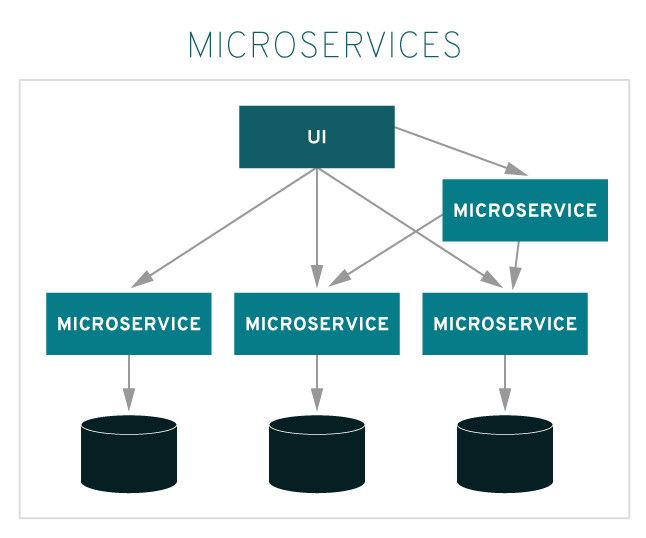
\includegraphics[width=0.55\textwidth]{monolithic-vs-microservices_altered.png}
            \caption{Structure of Microservices - [Altered], \\\textit{Source:~\cite{redhat_micro}}}\label{fig::micro}
        \end{figure}

        \subsubsection{Virtualization and Containerization}\label{sssec::virtual}
        Virtualization is an abstraction layer. The physical hardware (host) runs a hypervisor that allows the execution of (multiple) virtual machines (guests), which act like a regular computer~\cite{vmbasics}. This approach allows the usage of heterogeneous hardware without an impact on the guest operating systems due to the abstraction provided by the hypervisor. Without the need for specialized hardware and the dynamic allocation of resources, efficiency is increased~\cite{redhat_venv}. Additionally, virtual systems can be managed more easily because they are fundamentally just one big file on the host's storage device. They can be created on command, cloned and deleted without the configuration steps of a physical system. In the enterprise industry it is common to use this flexibility to start additional \ac{VM}s on high load. According to a study by the \ac{IDC} more than 80\% of data center workloads are virtualized~\cite{virtualaddoption}. Virtualization comes with the benefit of security. The majority of hypervisors strictly separate the host and the guest system in that the guest system is not allowed to use the hosts resources and access its files unless it is explicitly configured to do so. Compromising a \ac{VM} does not affect the host or any other \ac{VM}s~\cite{vmbasics},~\cite{redhat_venv}.\newline
        Full guest virtualization emulates a complete \ac{OS}, including the kernel, system libraries and even the majority of hardware devices. This abstraction comes with a performance penalty called overhead~\cite{vmbasics}. A supposedly more lightweight approach of virtualization is called containerization. Studies by Ericsson Research, Nomadic Lab~\cite{ieee_perfomance} and the Zhengzhou University~\cite{zhengzhou_university} conclude that, in fact, container based virtualization solutions provide better performance, especially in disk \acs{I/O} and network \acs{I/O} bound scenarios. Containerization focuses on the isolation of a single application process in a virtual runtime using control groups and namespace technology~\cite{cgroups}. Unlike \ac{VM}s, system and kernel functions are not virtualized and are passed through to the host machine. Consequently, overhead is reduced and allow the ability to run additional application instances compared to a \ac{VM}-based approach with the same amount of compute resources. Figure~\ref{fig::vm_docker} visualizes the differences between these approaches. The left side shows a traditional \ac{VM}-based approach. On top of the host \ac{OS} runs a hypervisor which provides three full guest \acl{OS}s with one application each. Each guest is fully isolated and features its own kernel, \ac{OS} and runtime libraries. The container-based solution on the right side only needs the host \ac{OS} and provides multiple application instances with shared libraries and runtimes in separated, isolated namespaces.\newline
        Apart from the performance benefits, the presumably main advantage of containers is their scalability, due to faster creation and startup times, which is what makes them an adequate fit for microservices \cite{cintainer_scale}. Docker, Podman and LXC are, amongst others, the most popular container-based virtualization solutions. A more detailed explanation of Docker can be found in Section~\ref{sssec::docker}.

        \begin{figure}
            \centering
            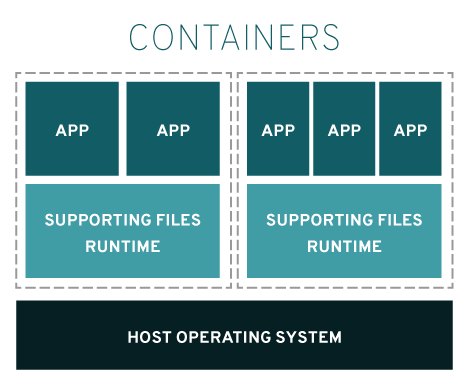
\includegraphics[width=0.9\textwidth]{docker-vm-redhat.png}
            \caption{Comparison of \ac{VM}s to Containers, \\\textit{Source:~\cite{redhat_pic}}}\label{fig::vm_docker}
        \end{figure}

        \subsubsection{Usage of Containerization in Microservices}
        As described above, microservices are small, bounded applications that communicate with each other. In order to follow the principles of loose coupling between applications, the communication should be performed via a protocol independent of the programming language. Typical IP based protocols used are \wordhighlight{\ac{REST}}, \wordhighlight{WebSockets} or \wordhighlight{GraphQL}~\cite{micro}. These loose-coupled applications have the advantage of being able to be developed simultaneously from different teams as well as upgraded and replaced independently. As a result, applications can be developed much faster and more flexible, following the principles of agile development~\cite{micro},~\cite{redhat_micro}.\newline
        The usage of containers drives this speed and flexibility even further. Containers provide a consistent and  isolated, yet flexible runtime for applications \cite{micro_container}. Applications are packaged within known good runtimes. This reduces the setup time of the deployment and eliminates host-specific errors. New application instances can be started without additional configuration. As a result of these successful concepts, tools like \wordhighlight{Docker Swarm} and \wordhighlight{Kubernetes} have been developed which can scale distributed applications in a managed dynamic, even automatic, way.\newline
        Packaging and eventually deploying the application introduce additional work for developers, which was previously a task of the operations team. As already stated above, the developer and the operations team are not separated in a DevOps culture. This approach values team communication, flexibility and autonomy, enabled by the structured, automated workflows between the development and operation tasks~\cite{effective_devops}. Eliminating manual tasks allows developers to focus on the actual application development. One of the main concepts in this process is the usage of \ac{CI} and \ac{CD} workflows.

    \subsection{Tools for Achieving a DevOps Environment}\label{ssec::getting_devops}
    Continuous integration and continuous deployment are two working concepts particularly well known in a \ac{MSA}. Since every application only provides one part of the overall service functionality, it is uncertain what effects a change in one application has on other applications and on the whole service. Accordingly, testing must take place between applications, especially if they are developed by different teams. This requires workflows checking these changes and simplifying recurring tasks through automation. For this purpose, explicit concepts and programs, which will also be used in the later Symbic project are presented below.

        \subsubsection{Version Control}
        A \acl{VCS} (\ac{VCS}) is an essential tool in the software development industry to keep track of which change has been made when and by whom. Contact persons for specific code sections are thus directly known and the responsibilities are clearly defined. \wordhighlight{Git} has become the de facto standard over the last 10 years and is also used in the following sample project, just like by over 93\% of all developers according to the StackOverflow Developer Survey 2021~\cite{stackoverflow2018}. Git allows collaborative, distributed work in own branches without affecting others. Changes can easily be merged back into the main branch, after an optional review has approved the changes. The new code is then made available for all developers. In the Symbic project, these functionalities are provided by a self-hosted instance of \wordhighlight{GitLab}. This is a service used to coordinate teamwork via issues and to document the project. Additionally, it serves as a central code repository. Its adaptability, extensive integration options and built-in \acs{CI} tools provide all the necessary software lifecycle programs from a single service bundle \cite{gitlabdocs}. \wordhighlight{GitHub} and \wordhighlight{Bitbucket} are alternatives, both of which offer code hosting, issue management, and \ac{CI}/\ac{CD}.

        \subsubsection{Continuous Integration}
        Continuous Integration is a practice in which new code is regularly integrated into the main code branch and into the overall service. Instead of having isolated functional branches that are worked on independently for months, changes flow back regularly into the main code branch to ensure it is free from conflicts and errors. Especially in interconnected services, it is indispensable to ensure that a change in one application do not have an unintended effect on other applications. \ac{CI} systems can perform automatic tasks, called jobs, on the code when it is checked into the \ac{VCS} repository. These tasks can ensure a specific code-style, run Unit or \acs{API}-tests and can also run integration tests against other services. If a task fails, the corresponding developer is notified and the changes are not incorporated into the main development branch. In case of an error, it becomes easier to identify its source due to these small and continuous integrations. Accordingly, errors and their causes can be identified more quickly and resolved without delay \cite{azuredevops}, \cite{base_devops}.\newline
        Popular services providing continuous integration functionality are \wordhighlight{Travis}, \wordhighlight{CircleCI}, \wordhighlight{GitHub Actions} and the previously mentioned GitLab \ac{CI}. These services differ in their function range, type of job configuration, the level of control, in their pricing models, or the number of free jobs, respectively, and in whether they can be self-hosted.

        \subsubsection{Continuous Deployment}
        Continuous deployment, on the other hand, is a practice bringing these regular updates into production quickly and automatically, making them available for customers, respectively. It typically involves two steps, continuous delivery and continuous deployment. The continuous creation of software bundles, which are called artifacts, falls under Continuous Delivery. The transfer of these artifacts and the process of making them usable is described as Continuous Deployment. To ensure product quality, it is best to have multiple deployment environments, as described in section \ref{ssec::devops_princibles}. Each new version is automatically deployed to a test or development environment, in which it undergoes automatic or manual testing. Common test types are security scans, load-, usability-, and acceptance tests. If all tests are successful, the version is promoted to the next deployment environment. In case of an error, the version is discontinued, and the developers get the corresponding notification. Only if none of the testing environments reveal any errors, the version will be transferred to production as a new release. \ac{CD} is an extension of the \ac{CI} principle and represents the next logical step in the software development workflow, which is why \ac{CI}/\ac{CD} are often used together \cite{azuredevops}. Well known \ac{CD} solutions are \wordhighlight{Jenkins}, \wordhighlight{Azure Pipelines}, \wordhighlight{\ac{AWS} CodeDeploy} and \wordhighlight{Argo \ac{CD}}.

        \subsubsection{Building a Streamlined Workflow}
        By combining these principles mentioned above, powerful workflows can be created that accelerate software development through automation and ensure consistent quality \cite{base_devops}. Figure~\ref{fig::cd} visualizes a complete exemplary \ac{CI}/\ac{CD} pipeline. It is typically built from multiple stages, each of those stages bundles one or more related tasks. A stage gets triggered by an event, such as code check-in or a previously successful stage. Common tasks are code style tests just as unit tests, automatic compilation or packaging and the deployment to a test system \cite{azuredevops}.\newline
        Both \ac{CI} and \ac{CD} are practices to automate tasks that have previously been performed manually. Integration testing and packaging both happen within the scope of a dedicated, autonomous system, which gives developers and operators more time for other activities. Deploying and using such a system are typical tasks in a DevOps practicing team. Here, the focus is on collaboration between the development and operations teams. At times new services must be added to the pipeline or existing services must be adapted to the current development status, depending on the current task. This workflow allows a team to react quickly and flexibly to changes and thus to comply with the agile principles. In collaborating closely and developing these well-functioning systems, the main goal is to add value to the product and to customer experience \cite{azuredevops}.\newline
        The GitLab instance, as used in the following project, serves to automatically test, build and deploy the code to a testing environment. Docker images are used to bundle the individual applications, which are explained in the next section. Thus, the built-in private image registry of GitLab also allows the creation of always up-to-date Docker images and makes them accessible to all authorized entities \cite{gitlabdocs}.
        % !TeX root = ../thesis_main.tex
\begin{figure}[]
    \centering
    \tikzstyle{block} = [rectangle, draw, fill=green!80!blue!70,
    text width=5em, text centered, rounded corners, minimum height=4em]
    \tikzstyle{line} = [draw, very thick, color=black!50, -latex']

    \begin{tikzpicture}[scale=2, node distance = 5cm, auto]
        % Place nodes
        \node [block] (init) {Code Check-in};
        \node [block, right of=init] (test) {\ac{CI} Pipeline \& Code-Test};
        \node [block, right of=test] (build) {Build \& Package Code};
        \node [block, below of=build, node distance=3.5cm] (d_test) {Deploy to Testing};
        \node [block, left of=d_test] (d_staging) {Deploy to Staging};
        \node [block, left of=d_staging] (d_live) {Deploy to Production};

        % Draw edges
        \path [line] (init) -- node {Triggers} (test);
        \path [line] (test) -- node {If successful} (build);
        \path [line] (build) -- node [left]{If successful} (d_test);
        \path [line] (d_test) -- node [above]{On approval} (d_staging);
        \path [line] (d_staging) -- node [text width=2.5cm, align=center, above]{On release approval} (d_live);
    \end{tikzpicture}
    \caption{Continuous Deployment Workflow, \\\textit{Source: Modeled after~\cite{azuredevops}}}
    \label{fig::cd}
\end{figure}



        \subsubsection{Containerization with Docker}\label{sssec::docker}
        In order to use the containerization concepts described in section \ref{sssec::virtual}, they have to be implemented in software. One solution for the implementation of container-based virtualization is Docker. Currently, Docker is the most popular containerization platform that is supported on Linux, Windows and macOS~\cite{docker_share}. It utilizes the Linux kernel of the host and its cgroups functionality for resource isolation. On none Linux host systems, Docker virtualizes the kernel via a built-in hypervisor. Docker was chosen for its wide usage, extensive documentation and its platform independency, which enables the usage in a local and productive operation.\newline
        Docker allows the isolated execution of applications within a container in a well-defined state without affecting the host. The initial state of a container is defined in a disk-image that bundles all the software, libraries and configuration files needed. Images are built based on a \wordhighlight{Dockerfile} that contains sequential, imperative instructions on how the container \ac{OS} should be configured. An exemplary Dockerfile can be found in the appendix in Listing \ref{code::docker}. Common steps are the \code{COPY} command to add files from the host to the container and the \code{RUN} command to execute shell commands within the container. Each file-changing instruction adds another layer to the overlay-filesystem that is used by Docker. Effectively making each layer a read only filesystem once it is written. At runtime, a file-lookup is performed in the top filesystem layer; lookups in the layers below follow if the file is not found in the first one. This allows the reuse of layers, because changed versions of files are simply pushed into a new layer and overshadow the original files. Images are usually kept as narrow as possible, so that they can be transferred more quickly and  present less a target, when it comes to matters of security. Therefore, only the minimum of necessary programs are provided in an image. Docker images are distributed via a registry to other systems. The company which develops Docker provides an official and public Docker image registry called \wordhighlight{DockerHub}. It offers official images of common applications, such as \acl{DB}s and webservers, as well as base images for own projects \cite{docker2020}, \cite{dockerdocs}.\newpage
        % !TeX root = ../thesis_main.tex

\begin{lstlisting}[language=docker, frame=single, caption={Exemplary NodeJS Dockerfile},label=code::docker]
# The base image to start from
FROM ubuntu:18

# Install nodeJS
RUN apt-get update && apt-get install -y nodejs npm

# Copy content of the Hosts "backend" folder to "app"
COPY ./backend /app

# Install all node-modules
RUN npm install

# Specifies the command that is executed at container start
ENTRYPOINT [ "npm", "start" ]

\end{lstlisting}

        When a container is started, the program specified in the image is executed, and the container runs until the started program exits. Each container is treated as an independent full-fledged computer with its own \ac{OS}. For this reason, each container has its own IP address and is by default not accessible from the host system. The user has to explicitly expose a container port to the host system in order to access the application inside the container. Each container does not only have its own IP address, but is also on its own virtual, software-defined network, which is managed by Docker and even uses a \ac{DNS} server that is inherent to Docker. Accordingly, containers within a defined network can communicate with each other by their (host-) names and provide their functionality outside the network by exposing their published ports to the host \ac{OS} \cite{docker2020}.\newline
        Unlike \ac{VM}s, the container's guest \ac{OS} is not maintained, as containers are considered disposable. Instead of updating the software within the container, it is simply replaced by a newer one from an updated image. All changes and new files within the old container are irreversibly lost. In order to avoid the loss of user data, private keys and the like, corresponding files can be stored persistent on the host system and made available in the container via mounts. A mounted directory behaves like a new top layer in the containers overlay filesystem. Docker distinguishes between volume-mounts and bind-mounts. Volumes are managed by Docker, have a unique name, can easily be shared between containers and are transferable between hosts whereas, in the case of bind-mounts, a specified directory is mounted from the host to the container. All filesystem attributes and file properties are passed on to the container, while their management is up to the user \cite{docker2020}, \cite{dockerdocs}.\newline
        Alternatives to Docker are \wordhighlight{Podman}, \wordhighlight{Rkt} and \wordhighlight{LXC}, which Docker was originally based on. The downside of these tools are their lower degree of integrability and lack of multi-platform support.

    \subsection{Relevance of Modern Development Techniques}
    The concepts explained above are becoming more and more relevant with the increasing adoption of agile principles, even outside the software industry. The annual agile report shows a significant growth in agile adoption from 37\% in 2020 to 86\% in 2021. The main reason for adopting agile practices seem to be enhanced ability to manage changing priorities and an increased speed of software delivery. Customers benefit from new features directly and developers receive immediate feedback. The same reasons for adopting agile also apply to the investment in a DevOps culture. The annual survey reveals, that more than 70\% of all respondents, are executing or planning a DevOps initiative. One of the biggest challenges in implementing DevOps seems to be inconsistencies in processes and practices, which is also reflected in the fragmented and heterogeneous processes described in the next section \cite{agilereport2021}.
